% !TeX document-id = {d42653b9-9ea4-48c2-860b-3d6e6e9d8ab0}
% !TeX TXS-program:compile = txs:///pdflatex/[--shell-escape]
\documentclass[12pt]{article} % For LaTeX2e
%\usepackage{neurips_2021}
\usepackage[colorlinks, citecolor={blue}]{hyperref}
\usepackage{url}
\usepackage{amsfonts,amscd,amssymb}
\usepackage{amsthm,amsmath,natbib}
\usepackage{algorithm,algorithmicx,algpseudocode}
\usepackage{bm}
\usepackage{bbm} %bb font numbers
\usepackage[table]{xcolor}
\usepackage{verbatim}
\usepackage{graphicx}
\usepackage{setspace}
\usepackage{natbib}
\usepackage[margin=1in]{geometry}
\usepackage{enumitem}
%\usepackage[nolists]{endfloat}
\usepackage{listings}
\usepackage[textsize=tiny]{todonotes}
\usepackage{tikz}
\usetikzlibrary{shapes.misc}
\usepackage{etoolbox}
\usepackage{appendix}
\usepackage[format=plain,
labelfont={it},
textfont=it]{caption}
\usepackage{subcaption}
\usepackage{wrapfig}
\usepackage{xr}
\usepackage{booktabs}
\usepackage{multirow}
\usepackage{authblk}
\usepackage{mathbbol}
\usepackage{thmtools}
\usepackage{amsfonts}



\usetikzlibrary{matrix}
\usetikzlibrary{backgrounds}
\usetikzlibrary{calc}
\usetikzlibrary{arrows,shapes}
\usetikzlibrary{decorations}
\usetikzlibrary{decorations.pathmorphing}
\usetikzlibrary{fit}
\usetikzlibrary{decorations.pathreplacing}
\usetikzlibrary{shapes.misc}
\usetikzlibrary{shapes.geometric}

\newtoggle{quickdraw}
%\toggletrue{quickdraw} % Uncomment this to render more quickly (non-random)


\definecolor{lightgrey}{rgb}{0.9,0.9,0.9}
\definecolor{darkgreen}{rgb}{0,0.3,0}
%\definecolor{darkred}{rgb}{0.3,0,0}

\definecolorset{rgb}{}{}{darkred,0.8,0,0;darkgreen,0,0.5,0;darkblue,0,0,0.5}

%\doublespacing

\newtheorem{thm}{Theorem}
\newtheorem{lemma}{Lemma}
\newtheorem{prop}{Proposition}
\newtheorem{cor}{Corollary}
\newtheorem{remark}{Remark}
\newtheorem{example}{Example}
\newtheorem{mydef}{Definition}
\newtheorem*{assumption}{Assumption}
\newtheorem{clm}{Claim}

\newcommand{\argmax}{\operatornamewithlimits{arg\,max}}
\newcommand{\argmin}{\operatornamewithlimits{arg\,min}}
\newcommand*{\fplus}{\genfrac{}{}{0pt}{}{}{+}}
\newcommand*{\fdots}{\genfrac{}{}{0pt}{}{}{\cdots}}
\newcommand{\mb}{\mathbf}
\newcommand{\mc}{\mathcal}
\newcommand{\dx}{\mbox{d}}

\renewcommand{\vec}[1]{\mathbf{#1}}
\newcommand{\numTaxa}{N}
\newcommand{\numTraits}{D}
\newcommand{\numDatasets}{M}
%\newcommand{\numLatent}{D}
\newcommand{\taxonIndex}{i}
\newcommand{\traitIndex}{j}
\newcommand{\traitData}{\vec{Y}}
\newcommand{\traitDatum}{y}
\newcommand{\datasetIndex}{m}
\newcommand{\exemplar}{\text{e}}

\newcommand{\sequences}{\vec{S}}
\newcommand{\latentData}{\vec{X}}
\newcommand{\latentdata}{\vec{x}}
\newcommand{\latentDatum}{x}
\newcommand{\phylogeneticParameters}{\boldsymbol{\phi}}
\newcommand{\phylogeny}{{\cal G}}
\newcommand{\tree}{\phylogeny}
%\newcommand{\otherParameters}{\boldsymbol{\
\newcommand{\transpose}{^{t}}

\newcommand{\distanceMatrix}{\mathbf{Y}}
\newcommand{\distance}{y}
\newcommand{\summant}{r}



\newcommand{\cdensity}[2]{\ensuremath{p(#1 \,|\,#2)}}
\newcommand{\density}[1]{\ensuremath{p(#1 )}}

\newcommand{\treeNode}{\nu}

\newcommand{\traitVariance}{\mathbf{\Sigma}}
\newcommand{\nodeIndex}{c}

%\newcommand{\parent}[1]{\mbox{\tiny pa}(#1)}
\newcommand{\parentBig}[1]{\mbox{pa}(#1)}

\newcommand{\sibling}[1]{\mbox{\tiny sib}(#1)}
\newcommand{\siblingBig}[1]{\mbox{sib}(#1)}

\newcommand{\rootMean}{\boldsymbol{\mu}_0}
\newcommand{\rootVarianceScalar}{\tau_0}
\newcommand{\unsequencedVarianceScalar}{\tau_{\exemplar}}
\newcommand{\treeVariance}{\vec{V}_{\tree}}
\newcommand{\hatTreeVariance}{\hat{\vec{V}}_{\tree}}
\newcommand{\mdsSD}{\sigma}
\newcommand{\mdsVariance}{\mdsSD^2}
\newcommand{\residual}{\hat{\traitDatum}}
\newcommand{\modelDistance}{\delta}
\newcommand{\cdf}{\phi}
\newcommand{\normalCDF}[1]{\Phi \left( #1 \right)}

\newcommand{\order}[1]{{\cal O}\hspace{-0.2em}\left( #1 \right)}

\newcommand{\rootNode}{\nu^{\datasetIndex}_{2 \numTaxa_{\datasetIndex} -1 }}
\newcommand{\pathLength}[1]{d(F, #1 )}
\newcommand{\pathLengthNew}[2]{
d_{F}
(
{#1}, {#2}
)
}
\newcommand{\J}{\vec{J}}
\newcommand{\pprime}{^{\prime}}
\newcommand{\otherIndex}{i \pprime}
\def\kronecker{\raisebox{1pt}{\ensuremath{\:\otimes\:}}}

\definecolor{trevorblue}{rgb}{0.330, 0.484, 0.828}
\definecolor{trevoryellow}{rgb}{0.829, 0.680, 0.306}


\allowdisplaybreaks

%\makeatletter
%\def\title@font{\Huge}
%\let\ltx@maketitle\@maketitle
%\def\@maketitle{\bgroup%
%	\let\ltx@title\@title%
%	\def\@title{\resizebox{\textwidth}{!}{%
%			\mbox{\title@font\ltx@title}%
%	}}%
%	\ltx@maketitle%
%	\egroup}
%\makeatother


\title{Approximating the matrix exponential derivative of the CTMC generator matrix, with application to global SARS-CoV-2}


%\date{}



\author[1]{Andrew J.~Holbrook}
\author[1]{Andrew F.~Magee}
\author[2]{Nathan E.~Glatt-Holtz}
\author[1,3,4]{Marc A.~Suchard}

 \affil[1]{Department of Biostatistics, University of California, Los Angeles}
 \affil[2]{Department of Mathematics, Tulane University}
 \affil[3]{Department of Biomathematics, University of California, Los Angeles}
 \affil[4]{Department of Human Genetics, University of California, Los Angeles}
 
 \renewcommand\Authands{ and }


\graphicspath{{figures/}}

\begin{document}


\maketitle




\begin{abstract}

We investigate the accuracy of a first-order approximation to the directional derivative of the matrix exponential evaluated on continuous-time Markov chain (CTMC) generator matrices.


\end{abstract}



\section{Introduction}\label{sec:intro}

%\newcommand{\x}{\mathbf{x}}
%\renewcommand{\v}{\mathbf{v}}

%\newcommand{\TTTheta}{\boldsymbol{\Theta}}
%\newcommand{\tr}{\mbox{tr}}
%\newcommand{\X}{\mathbf{X}}
%\renewcommand{\u}{\mathbf{u}}
\newcommand{\Y}{\mathbf{Y}}
\newcommand{\QQ}{\mathbf{Q}}
\newcommand{\DD}{\mathbf{D}}
\newcommand{\MM}{\mathbf{M}}
\newcommand{\JJ}{\mathbf{J}}
\newcommand{\II}{\mathbf{I}}
\newcommand{\RR}{\mathbf{R}}
%\newcommand{\haar}{\mathcal{H}}
%\newcommand{\orthog}{\mathcal{O}}
%\newcommand{\SSigma}{\boldsymbol{\Sigma}}
\newcommand{\Zero}{\boldsymbol{0}}
\newcommand{\ttheta}{\boldsymbol{\theta}}
\newcommand{\Llambda}{\boldsymbol{\Lambda}}
\newcommand{\vecc}{\mbox{vec}}
\newcommand{\CC}{\mathbf{C}}
\newcommand{\BB}{\mathbf{B}}
\renewcommand{\AA}{\mathbf{A}}
\newcommand{\GG}{\mathbf{G}}
\newcommand{\mom}{\boldsymbol{\xi}}

 We are interested in efficiently approximating the directional derivative of the matrix exponential
\begin{align*}
	e^{t\QQ} = \sum_{k=0}^\infty \frac{t^k\QQ^k}{k!}
\end{align*}
for arbitrary $t>0$ using the formula \citep{najfeld1995derivatives}
\begin{align}\label{eq:deriv}
	\nabla_{\JJ} e^{t\QQ}  =  e^{t\QQ}  \sum_{k=0}^\infty \frac{t^{k+1}}{(k+1)!} \{\JJ,\QQ^k\} \, .
\end{align}
Here, $\JJ$ gives the direction and $\{\JJ,\QQ^k\}$ is the matrix commutator series satisfying the recursion
\begin{align*}
	\{\JJ,\QQ^0\} &= \JJ \, , \\ 
	\{\JJ,\QQ^k\} &= [\{\JJ,\QQ^{k-1}\} , \QQ]  = \{\JJ,\QQ^{k-1}\} \QQ - \QQ \{\JJ,\QQ^{k-1}\} \, .
\end{align*}
Thus, the first-order approximation to derivative \eqref{eq:deriv} is 
\begin{align}\label{eq:firstOrder}
	\widetilde{\nabla}_{\JJ} e^{t\QQ}= t e^{t\QQ}\JJ \, .
\end{align}


\section{Global spread of SARS-CoV-2}


\begin{figure}[!t]
	\centering
	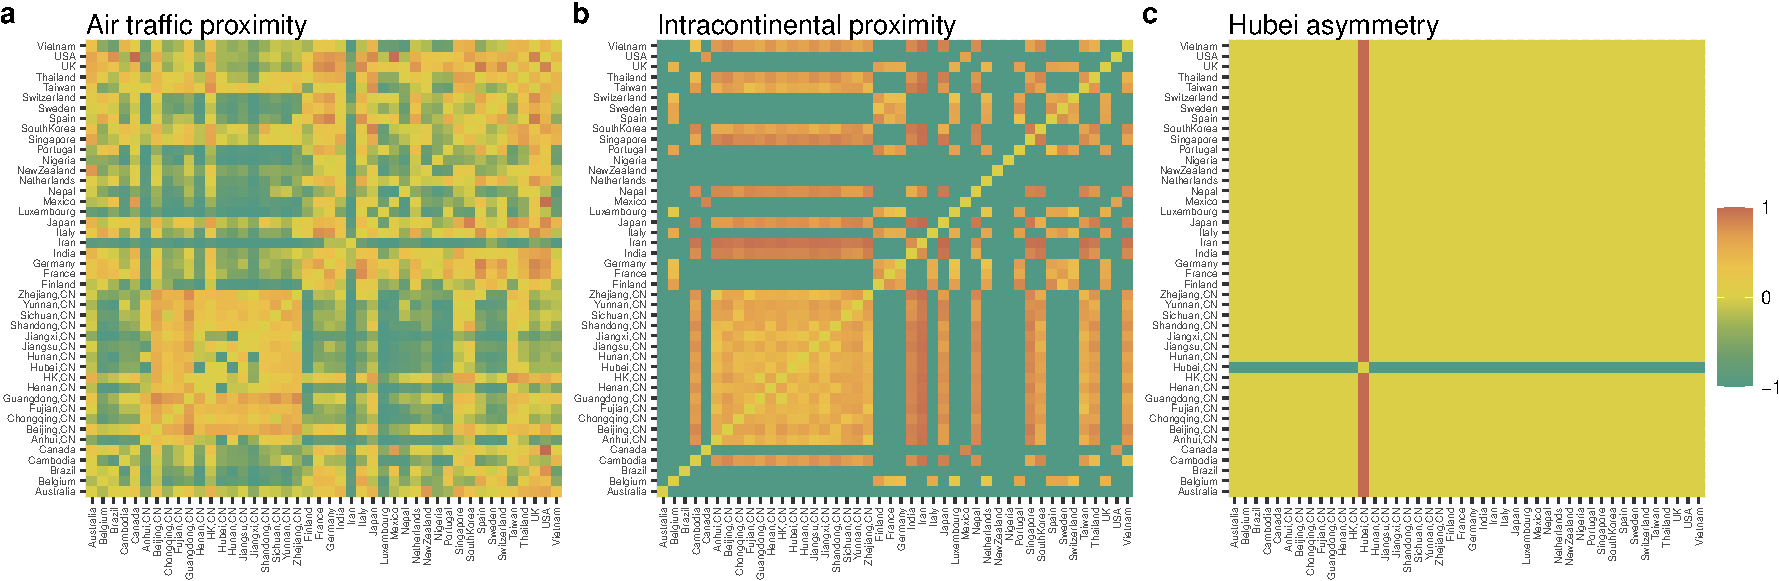
\includegraphics[width=\linewidth]{fixedEffects.pdf}
	\caption{Fixed effects.}\label{fig:FE}
\end{figure}

\begin{figure}[!t]
	\centering
	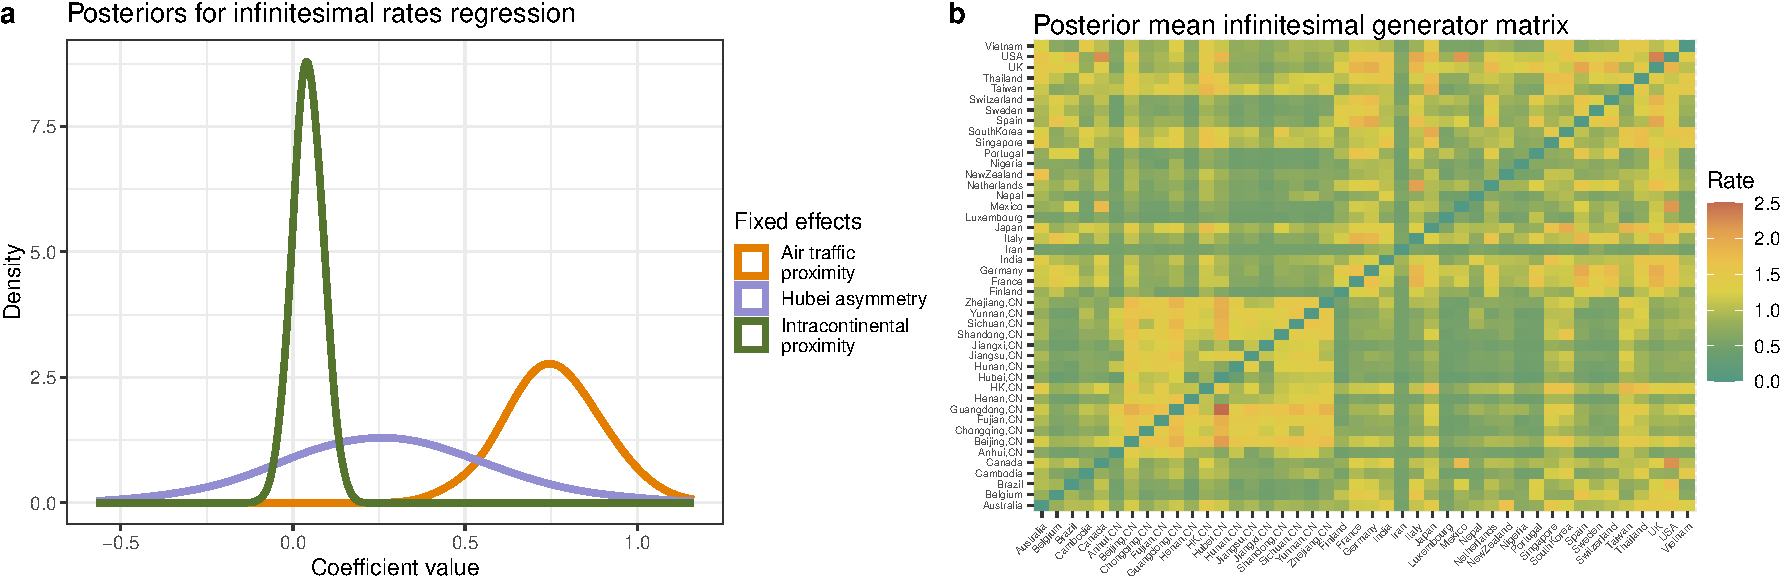
\includegraphics[width=\linewidth]{postViz.pdf}
	\caption{Posteriors.}\label{fig:FE}
\end{figure}

\subsection{Surrogate trajectory HMC}


Hamiltonian Monte Carlo (HMC) \citep{duane1987hybrid,neal2011mcmc} is an advanced MCMC procedure that uses numerical approximations to Hamiltonian trajectories to generate Metropolis-type \citep{metropolis1953equation} proposals far away from the current Markov chain state.  On the one hand, this approach to proposal generation helps reduce autocorrelation between chain states and is particularly helpful within higher-dimensional state spaces.  On the other hand, numerical integration of Hamilton's equations requires repeated evaluation of the Hamiltonian potential energy's gradient, and these repeated floating-point operations may become computationally burdensome.   Using HMC for Bayesian inference, the potential energy takes the form $u(\ttheta)=-\log \pi(\ttheta)$, where $\pi(\cdot)$ is the posterior density function $\pi(\ttheta):=p(\ttheta|\Y)$ of parameter $\ttheta\in\mathbb{R}^D$ given observed data $\Y$.  In this context, a single iteration of the the St\"{o}rmer-Verlet (velocity Verlet) or leapfrog integrator \citep{leimkuhler2004simulating}, beginning at time $\tau$ and with $\epsilon>0$ small, takes the form
\begin{align}\label{eq:leap}
	\mom\left(\tau + \frac{\epsilon}{2}\right) &= \mom(\tau) + \frac{\epsilon}{2} \nabla \log \pi(\ttheta(\tau))  \\  \nonumber
	\ttheta(\tau+\epsilon) &= \ttheta(\tau) + \epsilon \, \MM^{-1}\mom(\tau+\frac{\epsilon}{2}) \\ \nonumber
	\mom(\tau + \epsilon) &= \mom\left(\tau+\frac{\epsilon}{2}\right) + \frac{\epsilon}{2} \nabla \log \pi(\ttheta(\tau+\epsilon))  \, ,
\end{align}
where $\mom \sim \mbox{N}_D(\Zero,\MM)$ is the Hamiltonian system's Gaussian-distributed momentum variable.  
Different strategies aim to speed up the leapfrog integrator's many log-posterior gradient evaluations $\nabla \log \pi (\ttheta)$ in different ways, as these numerical routines often represent the algorithm's computational bottleneck.  In model-specific contexts, \citet{holbrook2021massive,holbrook2022bayesian,holbrook2022viral} develop parallelization strategies, and \citet{ji2020gradients} develop dynamic programming techniques, to accelerate $\nabla \log \pi (\ttheta)$.

A small body of work considers another approach by replacing $\nabla \log \pi (\ttheta)$ with a suitable approximation $\widehat{\nabla} \log \pi (\ttheta)$ and recognizing that the modified \eqref{eq:leap} continues to satisfy path reversibility and volume preservation, two essential ingredients for well-specified HMC. It follows immediately that the resulting `surrogate trajectory HMC' continues to sample the correct target distribution $\pi(\cdot)$.  Nonetheless, the acceptance rates and overall efficiency of such samplers may suffer when approximations are poor.   The majority of surrogate HMC methods first obtain a small sample of exact gradient evaluations and then use some model to interpolate: \citet{zhang2017precomputing} assume the approximate gradient follows a piecewise constant form across a grid; \citet{rasmussen2003gaussian,lan2016emulation} construct approximations using Gaussian processes; and \citet{zhang2017hamiltonian,li2019neural} do the same using neural networks.  But an even simpler approach to surrogate HMC may be appropriate when gradients have series representations.   \textcolor{red}{MAGEE} consider phylogenetic models that involve CTMC priors and show that the first-order approximation \eqref{eq:firstOrder} of the matrix exponential derivative \eqref{eq:deriv} performs remarkably well within surrogate HMC, achieving an over 30-fold efficiency gain compared to random-walk Metropolis for a 14-state model with over 180 model parameters.  Here, we demonstrate similar strong performance of the first-order approximation within surrogate HMC for a 44-state model with almost 1900 model parameters.



\subsection{Phylogeographic CTMC model}


\subsection{Bayesian analysis of SARS-CoV-2}


\section{Discussion}


\section*{Acknowledgments}

AJH is supported by a gift from the Karen Toffler Charitable Trust and by grants NIH K25 AI153816, NSF DMS 2152774 and NSF DMS 2236854.

%Let $\QQ=[q_{ij}]$ be the rate matrix for an $S$-dimensional continuous time Markov chain, where $q_{ij}>0$ for $i\neq j$, and $q_{ii} = -\sum_{j\neq i} q_{ij}$.  In our application of interest, $\QQ$ is almost surely diagonalizable, i.e., $\QQ=\MM \DD \MM^{-1}$ for 
%\begin{align*}
%	\DD = \begin{pmatrix}
%		d_1& 0 &\dots & & \\
%		0  & d_2 &0  & \dots& \\
%		\vdots &0 & \ddots & \\
%		& \vdots& & d_{S-1} &0 \\
%		&&&0&0
%	\end{pmatrix} \, ,
%\end{align*}
%where the structure of $\QQ$ implies eigenvalues
%\begin{enumerate}
%	\item $d_s\in \mathbb{C}$ with $\mbox{Re}(d_s)<0$ for $s\in\{1,\dots,S-1\}$, and
%	\item $d_S =0$ corresponding to the eigenvector $\boldsymbol{1}=(1,\dots,1)^T$. 
%\end{enumerate} 
%We may further define a generalized inverse $\QQ^+=\MM \DD^{+} \MM^{-1}$ of $\QQ$ using $\DD^+$, the Moore-Penrose pseudoinverse obtained by inverting the non-zero elements of $\DD$.   Finally, we note that diagonalizability implies $\DD$ and $\DD^+$ commute, i.e., $\DD^+\DD=\DD\DD^+$.
%
%
% We are interested in efficiently approximating the directional derivative of the matrix exponential
%\begin{align*}
%	e^{t\QQ} = \sum_{k=0}^\infty \frac{t^k\QQ^k}{k!}
%\end{align*}
%for arbitrary $t>0$ using the formula \citep{najfeld1995derivatives}
%\begin{align}\label{eq:deriv}
%	\nabla_{\JJ} e^{t\QQ}  =  e^{t\QQ}  \sum_{k=0}^\infty \frac{t^{k+1}}{(k+1)!} \{\JJ,\QQ^k\} \, .
%\end{align}
%Here, $\JJ$ gives the direction and $\{\JJ,\QQ^k\}$ is the matrix commutator series satisfying the recursion
%\begin{align*}
%	\{\JJ,\QQ^0\} &= \JJ \, , \\ 
%	\{\JJ,\QQ^k\} &= [\{\JJ,\QQ^{k-1}\} , \QQ]  = \{\JJ,\QQ^{k-1}\} \QQ - \QQ \{\JJ,\QQ^{k-1}\} \, .
%\end{align*}
%Thus, the first-order approximation to derivative \eqref{eq:deriv} is 
%\begin{align}\label{eq:firstOrder}
%	\widetilde{\nabla}_{\JJ} e^{t\QQ}= t e^{t\QQ}\JJ \, .
%\end{align}
%We want to bound the truncation error
%\begin{align*}
%\mbox{err}(t,\QQ,\JJ)	:=\lVert \nabla_{\JJ} e^{t\QQ} - \widetilde{\nabla}_{\JJ} e^{t\QQ} \rVert \, ,
%\end{align*}
% where $\lVert \cdot \rVert$ denotes an appropriate matrix norm.  In this context, we find that naive bounds (Appendix \ref{sec:loose}) that do not exploit the structure of $\QQ$  are rather loose (Figure \ref{fig:frob}).  
% In our efforts to fully leverage the structure of $\QQ$, we will make use of the general formula for the matrix commutator series  \citep{volkin1968iterated}
%\begin{align}\label{eq:commSeries}
%	\{ \JJ, \QQ^k\} = \sum_{r=0}^k (-1)^{k+r}  {k \choose r} \QQ^{k-r} \JJ \QQ^r  \, .
%\end{align}
%
%\subsection{An empirically tight asymptotic estimate}
%
%We begin by noting
%\begin{align}\label{eq:ub1}
%	\mbox{err}(t,\QQ,\JJ) &=  \lVert  e^{t\QQ}  \sum_{k=1}^\infty \frac{t^{k+1}}{(k+1)!} \{\JJ,\QQ^k\} \rVert \\ \nonumber
%	&\leq  \lVert  e^{t\QQ}\JJ  \sum_{k=1}^\infty \frac{t^{k+1}}{(k+1)!} \QQ^k \rVert +   \lVert  e^{t\QQ}  \sum_{k=1}^\infty \frac{t^{k+1}}{(k+1)!} \{\JJ,\QQ^k\} -\JJ\QQ^k\rVert \\ \nonumber
%		&=  \lVert  e^{t\QQ}\JJ \QQ^+  \sum_{k=1}^\infty \frac{t^{k+1}}{(k+1)!} \QQ^{k+1} \rVert +   \lVert  e^{t\QQ}  \sum_{k=1}^\infty \frac{t^{k+1}}{(k+1)!} \{\JJ,\QQ^k\} -\JJ\QQ^k\rVert \\ \nonumber
%		&=  \lVert  e^{t\QQ}\JJ \QQ^+ (e^{t\QQ} - t\QQ -\II) \rVert +   \lVert  e^{t\QQ}  \sum_{k=1}^\infty \frac{t^{k+1}}{(k+1)!} \{\JJ,\QQ^k\} -\JJ\QQ^k\rVert \\ \nonumber
%			&\leq \lVert  e^{t\QQ}\JJ \QQ^+ ( t\QQ +\II) \rVert  + \lVert  e^{t\QQ}\JJ \QQ^+ e^{t\QQ} \rVert  +   \lVert  e^{t\QQ}  \sum_{k=1}^\infty \frac{t^{k+1}}{(k+1)!} \{\JJ,\QQ^k\} -\JJ\QQ^k\rVert \\ \nonumber
%			&=: \mathfrak{a} + \mathfrak{b} + \mathfrak{c} \, .
%\end{align}
%Empirical experiments using the Frobenius and infinity norms (Figures \ref{fig:frob} and \ref{fig:inf}, respectively) show that the first term
%\begin{align}
%	 \mathfrak{a} = \left\Vert e^{t\QQ} \JJ \QQ^+(t\QQ+\II)  \right\Vert \, ,
%\end{align}
%although not a strict upper bound, is asymptotically tight for the true error as $t\rightarrow \infty$. We would, therefore, like to show that the terms $\mathfrak{b}$ and $\mathfrak{c}$ go to zero as $t$ diverges.
%
%
%
%
%
%
%
%
%\section{Using the structure of $\QQ$}
%
%We use the fact that
%\begin{align*}
%	e^{t\QQ}\QQ = \MM \exp(t\DD) \DD \MM^{-1} =  \MM \begin{pmatrix}
%	e^{td_1}	d_1& 0 &\dots & & \\
%		0  & e^{td_2}d_2 &0  & \dots& \\
%		\vdots &0 & \ddots & \\
%		& \vdots& & e^{td_{S-1}}d_{S-1} &0 \\
%		&&&0&0
%	\end{pmatrix} \MM^{-1} \, .
%\end{align*}
%Thus, assuming use of a submultiplicative norm leads to the result
%\begin{align*}
%	\lVert e^{t\QQ}\QQ \rVert &\leq \left\Vert  \begin{pmatrix}
%		e^{td_1}	d_1& 0 &\dots & & \\
%		0  & e^{td_2}d_2 &0  & \dots& \\
%		\vdots &0 & \ddots & \\
%		& \vdots& & e^{td_{S-1}}d_{S-1} &0 \\
%		&&&0&0
%	\end{pmatrix}  \right\Vert  \lVert \MM\rVert   \lVert \MM^{-1}\rVert  \, .
%\end{align*}
%For, e.g., the Frobenius norm, we have
%\begin{align*}
%\lVert e^{t\QQ}\QQ \rVert_F	\leq \sqrt{S-1} \max_s \{|e^{td_{s}} d_{s}| \}  \lVert \MM\rVert_F   \lVert \MM^{-1}\rVert_F  \, ,
%\end{align*}
%where we  use the fact that $\lVert \cdot \rVert_F \leq \sqrt{r} \lVert \cdot \rVert_2$ for any rank $r$ matrix and $\lVert \cdot \rVert_2$ the spectral norm.  We therefore write
%\begin{align}
%	\lVert e^{t\QQ}\QQ \rVert_F = \order{\max_s \left\{|e^{td_{s}} d_{s}| \right\}} \,,  \quad 	\lVert e^{t\QQ}\QQ^+ \rVert_F = \order{\max_s \left\{ \left| e^{td_{s}} \frac{1}{d_{s}}\right| \right\}} \, .
%\end{align}
%Because $\mbox{Re}(d_s)<0$ for $s\in \{1,\dots,S-1\}$, we have
%\begin{align}
%	\lim_{t\rightarrow \infty}  	\lVert e^{t\QQ}\QQ \rVert_F = 	\lim_{t\rightarrow \infty}  	\lVert e^{t\QQ}\QQ^+ \rVert_F = 0\, ,
%\end{align}
%and, by equivalence of norms, we have
%\begin{align}
%	\lim_{t\rightarrow \infty}  	\lVert e^{t\QQ}\QQ \rVert = 	\lim_{t\rightarrow \infty}  	\lVert e^{t\QQ}\QQ^+ \rVert = 0\, ,
%\end{align}
%in general for any matrix norm $\lVert \cdot \rVert$. Moreover, the matrix $e^{t\QQ}$ is a stochastic matrix with rows summing to unity. Therefore $\lVert e^{t\QQ}\rVert_\infty = 1$, and, by norm equivalence, $\lVert e^{t\QQ}\rVert = \mathcal{O}(1)$.
% These results lead to the following fact for term $\mathfrak{b}$ in the upper bound of \eqref{eq:ub1}:
%\begin{align*}
%	\lim_{t\rightarrow \infty} \lVert  e^{t\QQ}\JJ \QQ^+ e^{t\QQ} \rVert \leq  \lim_{t\rightarrow \infty} \lVert  e^{t\QQ} \rVert \lVert \JJ  \rVert \lVert \QQ^+ e^{t\QQ} \rVert = 0 \, .
%\end{align*}
%Thus, we obtain the intermediary result for $t$ large:
%\begin{align*}
%\lim_{t\rightarrow \infty}\mbox{err}(t,\QQ,\JJ) \leq \lim_{t\rightarrow \infty}  \mathfrak{a}+ \mathfrak{c} \, .
%\end{align*}
%It remains to show that $\mathfrak{c}$ goes to zero as $t$ diverges, i.e., 
%\begin{align}
%	\lim_{t\rightarrow \infty} \lVert  e^{t\QQ}  \sum_{k=1}^\infty \frac{t^{k+1}}{(k+1)!} \{\JJ,\QQ^k\} -\JJ\QQ^k\rVert = 0\, .
%\end{align}
%
%
%
%\section{Random thoughts}
%
%\subsection{Another form}
%
%\newcommand{\PPsi}{\boldsymbol{\Psi}}
%
%\citet{najfeld1995derivatives} use the integral representation to prove the interesting result
%\begin{align*}
%	\nabla_{\JJ} e^{t\QQ} = \MM \left(  \left(\MM^{-1} \JJ \MM\right) \circ \PPsi(t)  \right) \MM^{-1} \, ,
%\end{align*}
%where $\PPsi(t)$ has elements
%\begin{align*}
%		[\PPsi(t)]_{ij} = \bigg\{ \begin{array}{cc}
%		t e^{td_i}\, ,	&  d_i = d_j \\
%		\frac{e^{td_i}-e^{td_j}}{d_i-d_j} \, ,& d_i \neq d_j 
%	\end{array} \, .
%\end{align*}
%For our application, the eigenvalues equal one another with measure zero.  Taking $t$ large, we have
%\begin{align*}
%	[\PPsi(t)]_{ij} = \bigg\{ \begin{array}{cc}
%		t e^{td_i}\, ,	&  i = j \\
%		0 \, ,& i \neq j 
%	\end{array} \, .
%\end{align*}
%It follows that, again for $t$ large,
%\begin{align*}
%	\mbox{err}(t,\QQ,\JJ) &\approx \lVert   \MM \left(  \left(\MM^{-1} \JJ \MM\right) \circ t e^{t\DD}  \right) \MM^{-1}       -  t e^{t\QQ} \JJ            \rVert \\
%	&= t\lVert   \MM \rVert \lVert \left(  \left(\MM^{-1} \JJ \MM\right) \circ  e^{t\DD}  \right) \MM^{-1}       -   e^{t\DD}\MM^{-1} \JJ            \rVert \, .
%\end{align*}
%
%\appendix
%
%\section{Loose bounds}\label{sec:loose}
%
%The following loose bounds do not leverage the structure of the CTMC generator matrix $\QQ$.
%
%\subsection{Upper bound 1}
%
%
%
%For a submultiplicative matrix norm, we have
%\begin{align*}
%	\Vert \{\MM_1, \MM_2^k \}  \Vert \leq 2^k \Vert \MM_1\Vert \Vert\MM_2 \Vert ^k \, .
%\end{align*}
%We use this to obtain our first upper bound on $err_{ij}(\QQ)$:
%\begin{align*}
%	err_{ij}(\QQ) &= \left\Vert e^{t\QQ}  \sum_{k=1}^\infty \frac{t^{k+1}}{(k+1)!} \{\JJ,\QQ^k\} \right\Vert  \\
%	&\leq \Vert e^{t\QQ} \Vert \sum_{k=1}^\infty \left\Vert \frac{t^{k+1}}{(k+1)!} \{\JJ,\QQ^k\} \right\Vert  \\
%	&=  \Vert e^{t\QQ} \Vert \sum_{k=1}^\infty \frac{t}{k+1} \frac{(2t \Vert \QQ \Vert)^k}{k!}\\
%	&= \Vert e^{t\QQ} \Vert   \frac{\exp(2t\Vert \QQ \Vert)-2t\Vert\QQ\Vert-1}{2\Vert \QQ \Vert} 
%\end{align*}
%
%
%\subsection{Upper bound 2}
%
%We start with another representation of the derivative \citep{al2009computing}:
%\begin{align*}
%	\nabla_{\JJ} e^{t\QQ} = \sum_{k=1}^\infty \frac{t^k}{k!} \sum_{p=1}^k \QQ^{p-1} \JJ \QQ^{k-p} 
%\end{align*}
%and the fact that
%the fact that, for the Frobenius norm $\Vert \cdot \Vert_F$, we have \citep{wu2010short}
%\begin{align*}
%	\Vert [\MM_1,\MM_2] \Vert_F \leq \sqrt{2} \Vert \MM_1 \Vert_F \Vert \MM_2\Vert_F \, .
%\end{align*}
%Using these results, the truncation error may be rewritten
%\begin{align*}
%	err_{ij}(\QQ)  &=\left\Vert - te^{t\QQ} \JJ  +  \sum_{k=1}^\infty \frac{t^k}{k!} \sum_{p=1}^k \QQ^{p-1} \JJ \QQ^{k-p}\right\Vert_F \\
%	&= \left\Vert \sum_{k=1}^\infty \frac{t^k}{k!} \left( \left( \sum_{p=1}^k \QQ^{p-1} \JJ \QQ^{k-p} \right) - k \QQ^{k-1} \JJ \right)  \right\Vert_F\\
%	&= \left\Vert \sum_{k=1}^\infty \frac{t^k}{k!} \sum_{p=1}^k \QQ^{p-1} \JJ \QQ^{k-p}  -  \QQ^{k-1} \JJ \right\Vert_F \\
%	&=\left\Vert  \sum_{k=1}^\infty \frac{t^k}{k!} \sum_{p=1}^{k-1} \QQ^{p-1} \JJ \QQ^{k-p}  -  \QQ^{k-1} \JJ\right\Vert_F \\
%	&=\left\Vert  \sum_{k=1}^\infty \frac{t^k}{k!} \sum_{p=1}^{k-1} \QQ^{p-1}\left( \JJ \QQ^{k-p}  -  \QQ^{k-p} \JJ \right)\right\Vert_F \\
%	&= \left\Vert  \sum_{k=1}^\infty \frac{t^k}{k!} \sum_{p=1}^{k-1} \QQ^{p-1}[\JJ, \QQ^{k-p}] \right\Vert_F  \\
%	&\leq  \sum_{k=1}^\infty \frac{t^k}{k!} \sum_{p=1}^{k-1} \Vert \QQ^{p-1} \Vert_F \Vert[\JJ, \QQ^{k-p}]\Vert_F 
%	\leq \sqrt{2}  \sum_{k=1}^\infty \frac{t^k}{k!} \sum_{p=1}^{k-1} \Vert \QQ^{k-1} \Vert_F  \\
%	&= \sqrt{2}  \sum_{k=1}^\infty \frac{t^k}{k!} (k-1) \Vert \QQ \Vert_F^{k-1} = \sqrt{2} \frac{e^{t\Vert \QQ\Vert_F}(t\Vert\QQ\Vert_F - 1) + 1}{\Vert \QQ \Vert_F} \, .
%\end{align*}


%\begin{figure}[!p]
%	\centering
%	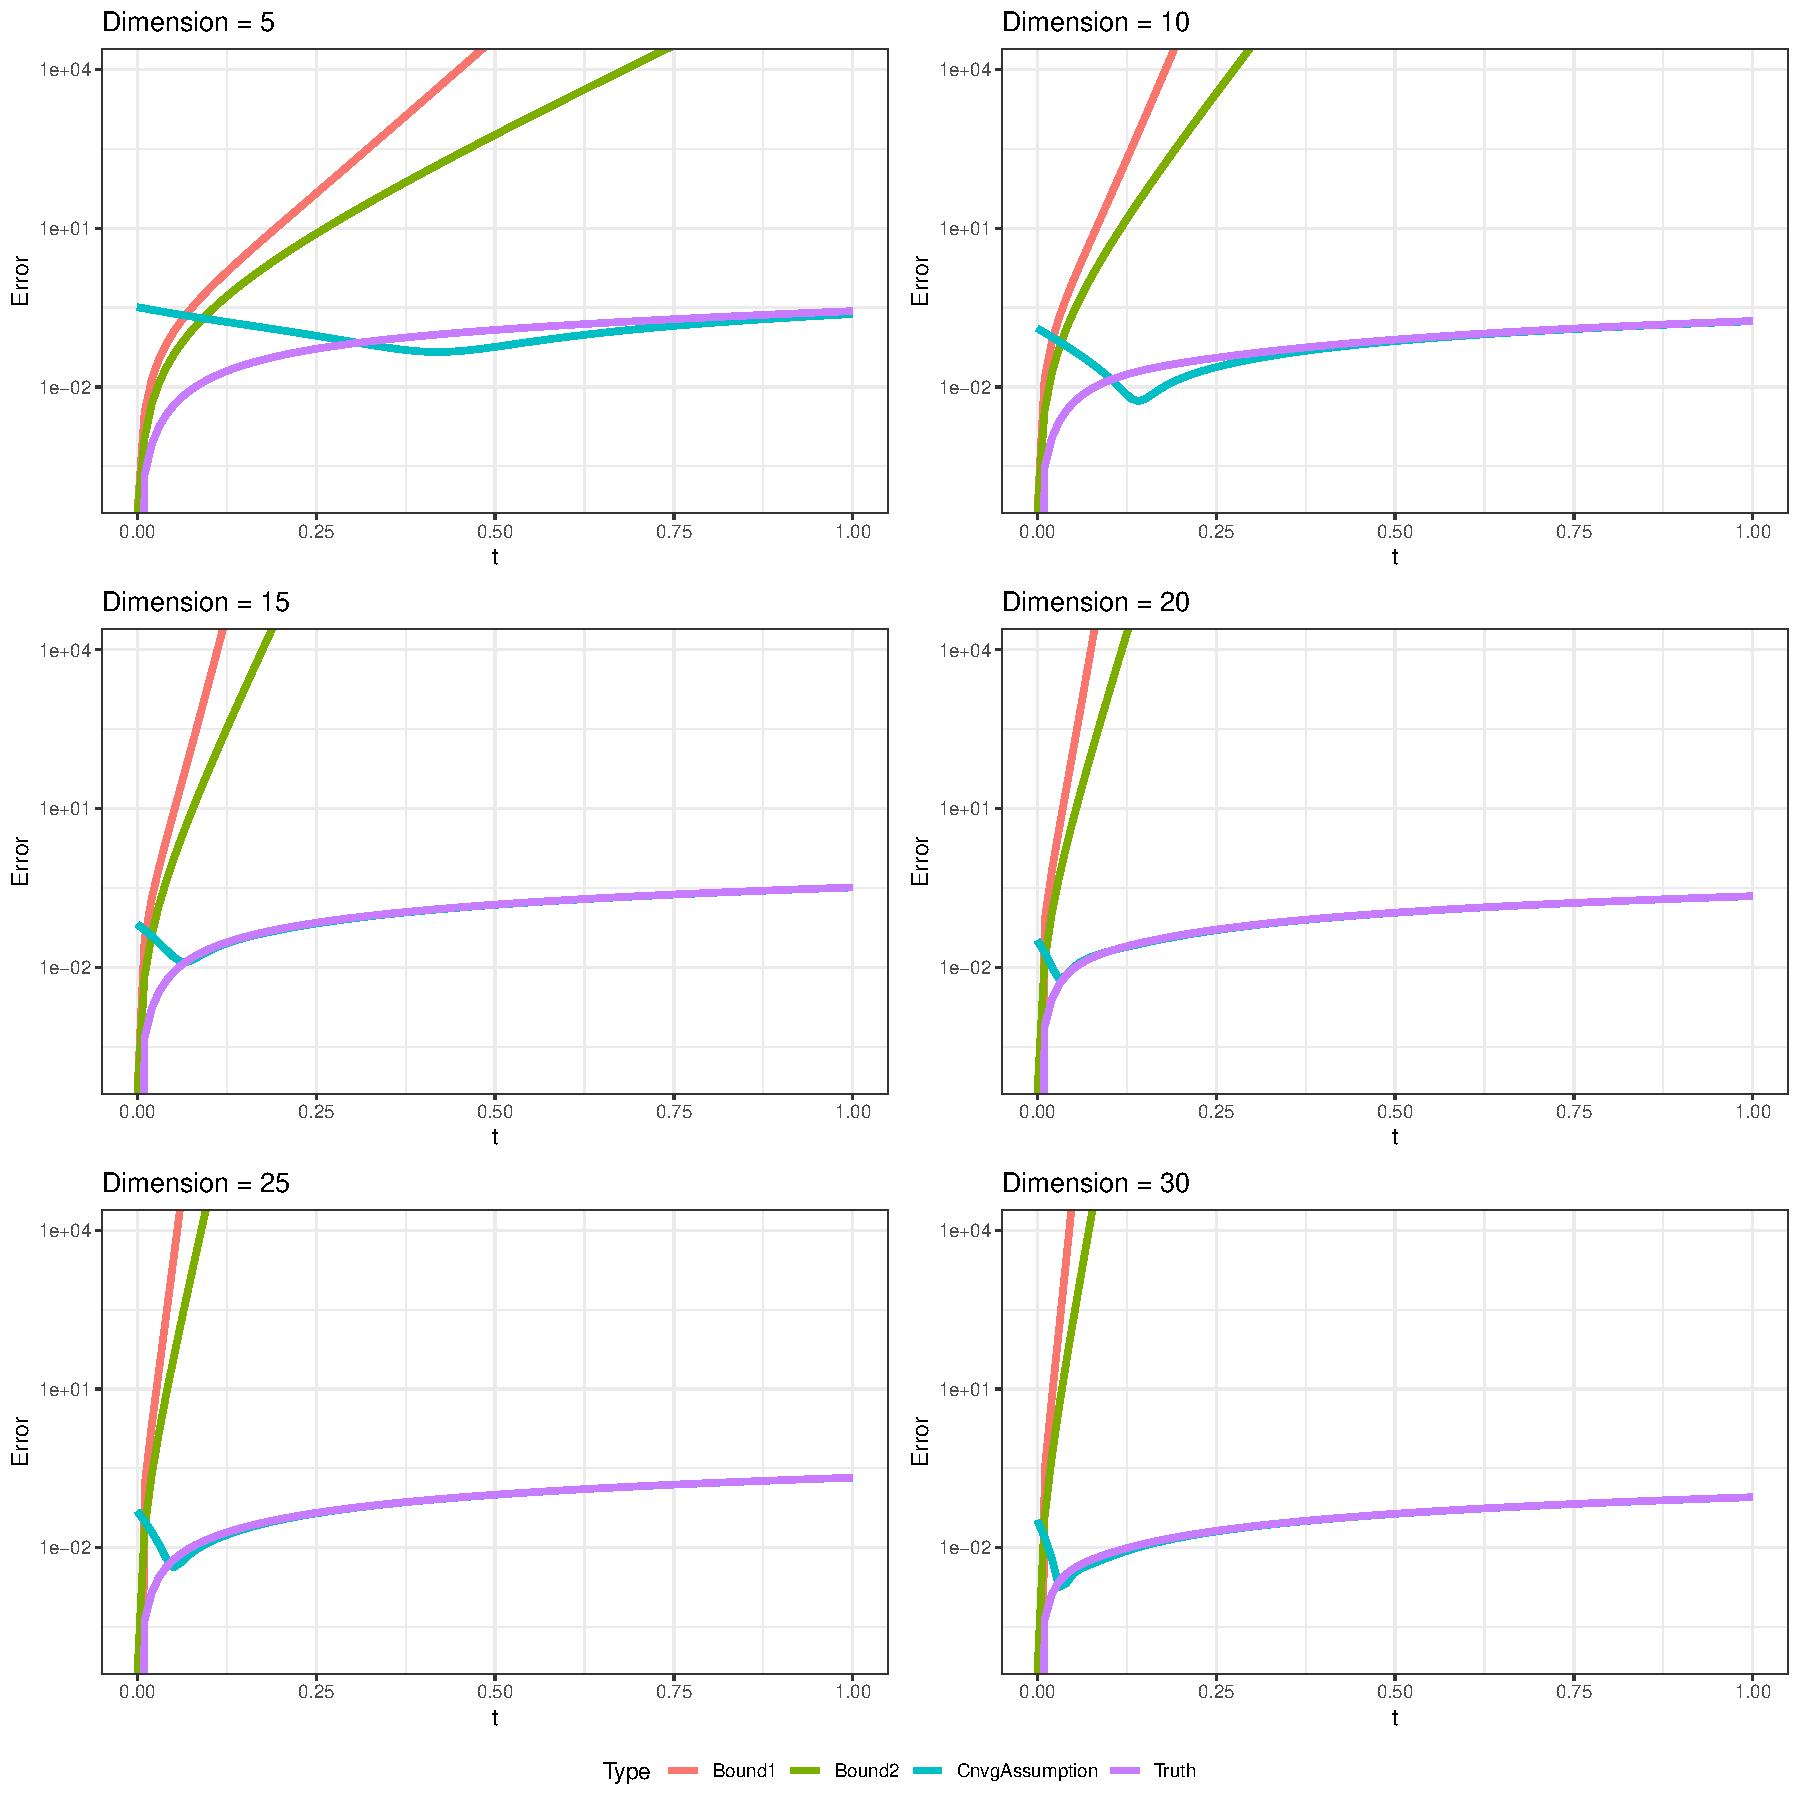
\includegraphics[width=\linewidth]{frobeniusScaling.pdf}
%	\caption{Anecdotal (single simulation) error profiles with change in time $t$ and dimension. Errors calculated using Frobenius norm.}\label{fig:frob}
%\end{figure}
%
%\begin{figure}[!p]
%	\centering
%	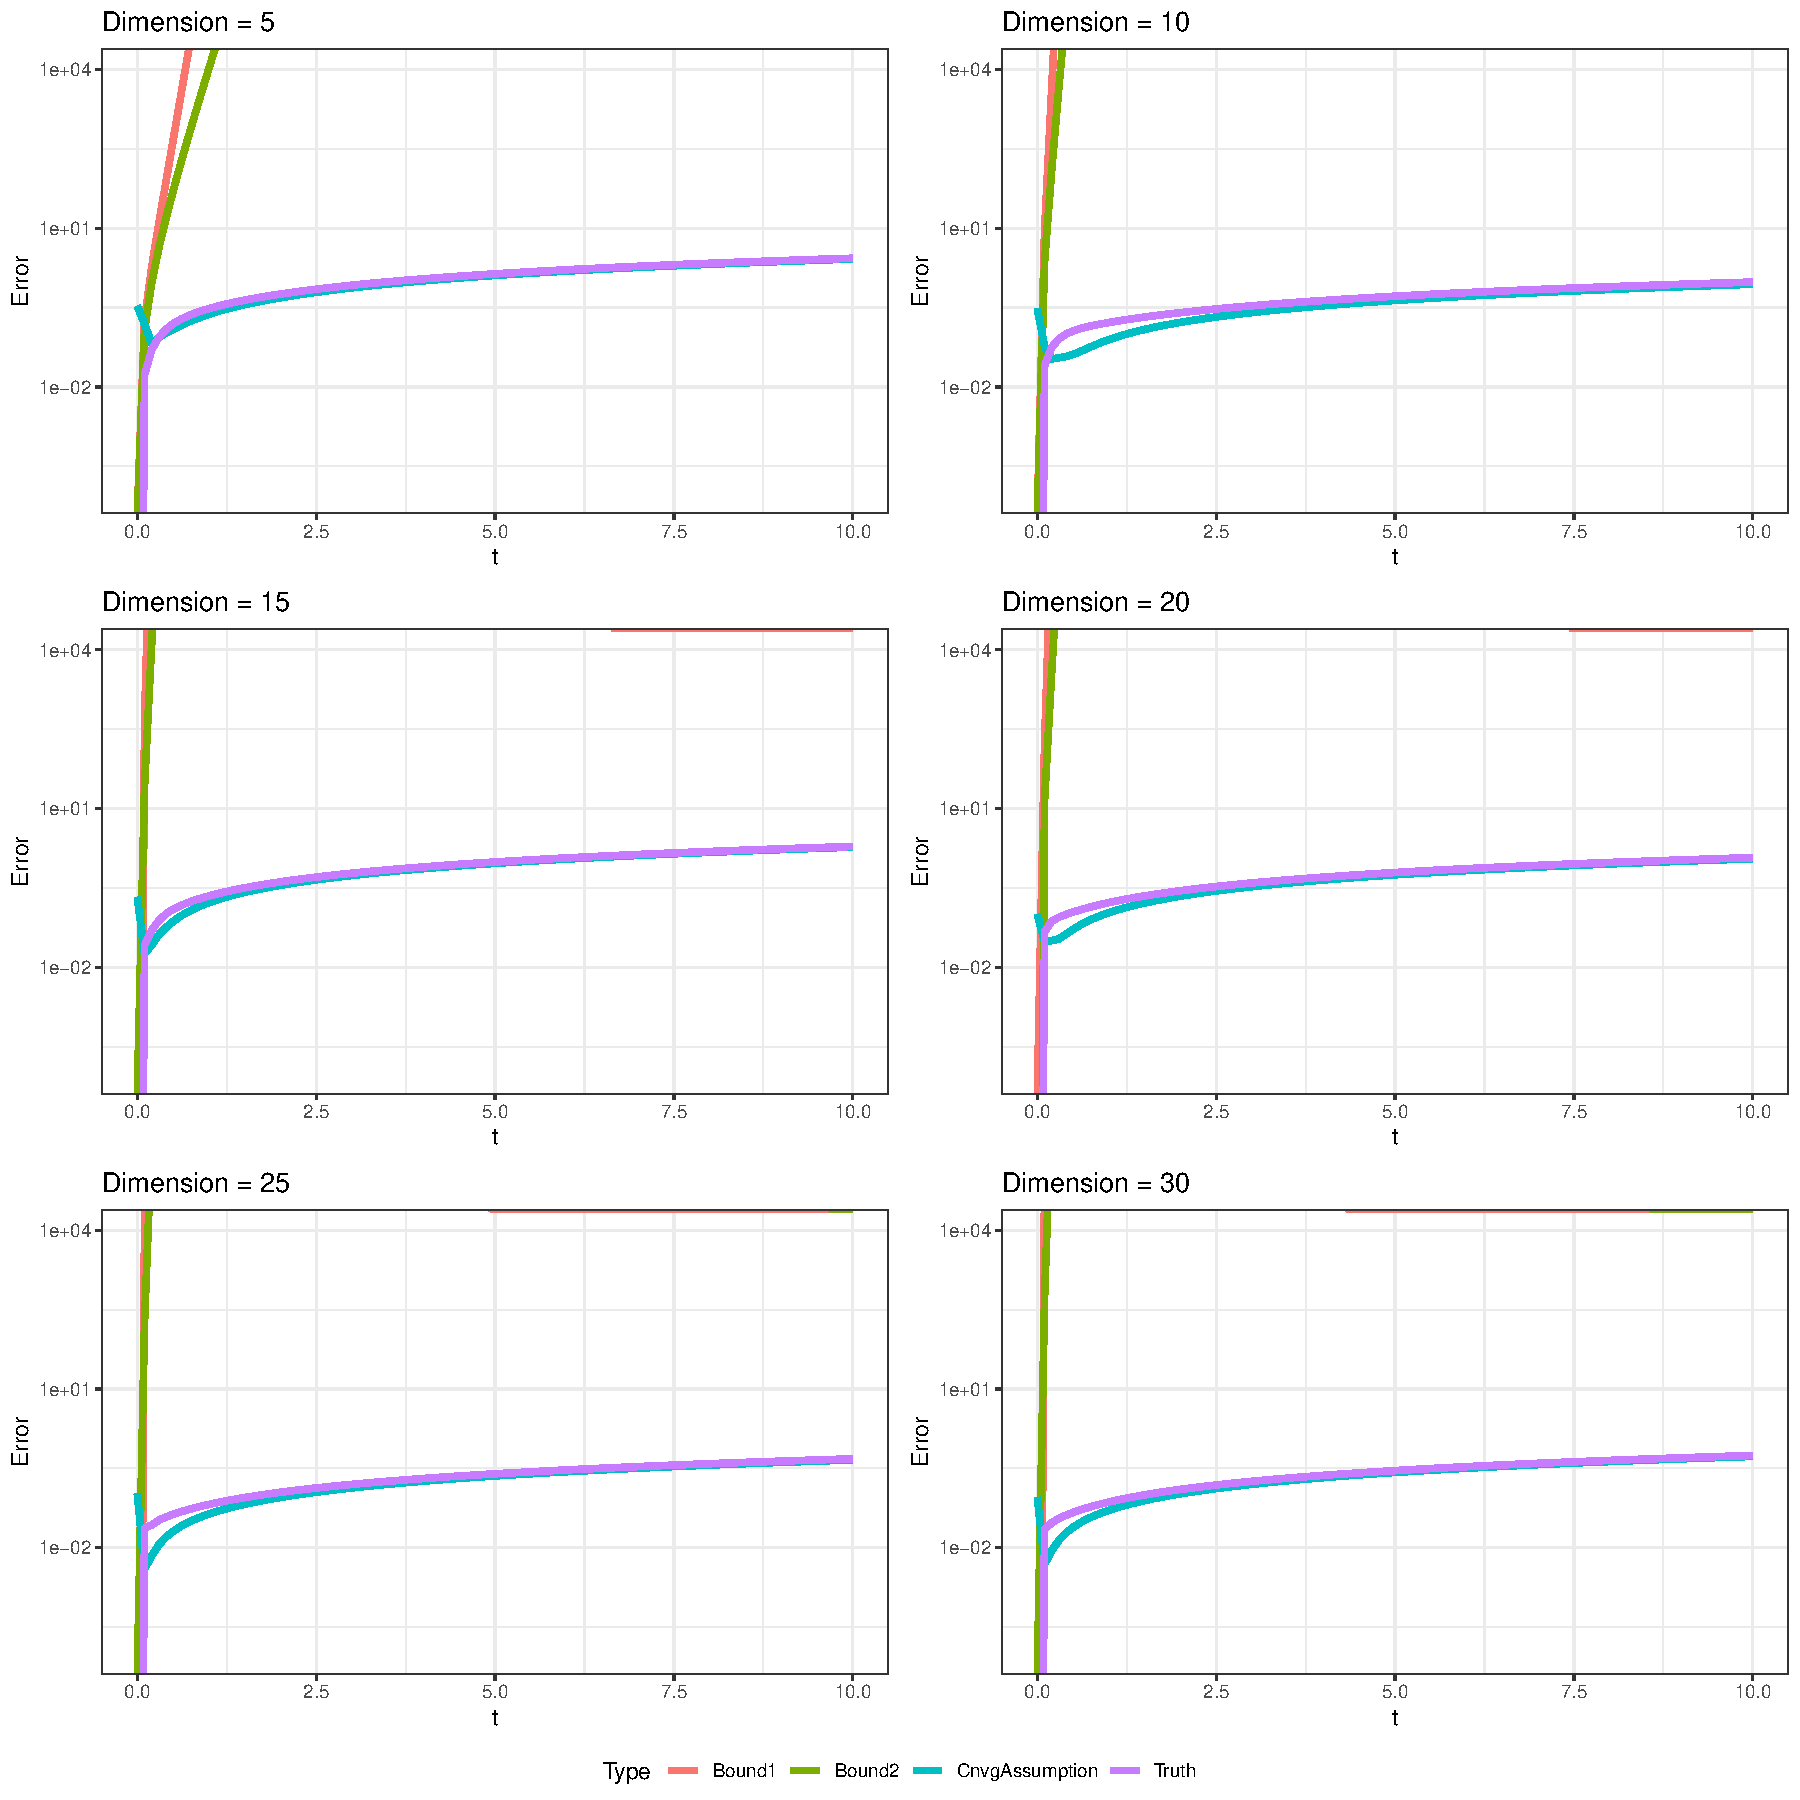
\includegraphics[width=\linewidth]{infinityScaling.pdf}
%	\caption{Anecdotal (single simulation) error profiles with change in time $t$ and dimension. Errors calculated using infinity norm.}\label{fig:inf}
%\end{figure}

\bibliographystyle{sysbio}
\bibliography{refs}


%%%%%%%%%%%%%%%%%%%%%%%%%%%%%%%%%%%%%%%%%%%%%%%%%%%%%%%%%%%%

\end{document}
